\[
\begin{array}{cc}
\hline
x_i & y_i \\
\hline
0 & 1 \\
1 & 2 \\
2 & 33 \\
3 & 244 \\
\hline
\end{array}
\]

\begin{table}[H]
\centering
\caption{Tabla de polos, ceros y estabilidad}
\label{tabla:estabilidad}
%\begin{tabular}{|p{15cm}|}
%%%%%%%%%%%%%%%%%%%%%%%%%%%%%%%%%%%%%%%%%%%%%%%%%%%%%%%%%%%%%%%%%%%%%%%%%%%%%%%%%%%%%%%%%%%%%
\begin{tabular}{llll}
\hline
\multicolumn{1}{c}{\textbf{G}} & \multicolumn{1}{c}{\textbf{Polos}} & \multicolumn{1}{c}{\textbf{Ceros}} & \multicolumn{1}{c}{\textbf{Estabilidad}} \\ \hline
\hyperref[CON1]{G2}                             &                                    &                                    &                                         
\end{tabular}
%%%%%%%%%%%%%%%%%%%%%%%%%%%%%%%%%%%%%%%%%%%%%%%%%%%%%%%%%%%%%%%%%%%%%%%%%%%%%%%%%%%%%%%%%%%%%
\end{table}
\textbf{}


\begin{enumerate}
    \item Encuentre el polinomio interpolante de Lagrange, grafique el polinomio y estime el valor de \( y \) que corresponde a \( x = 2.7 \).
    \item Construya el trazador cúbico, grafique el polinomio y estime el valor correspondiente para \( x = 2.7 \).
    \item Compare los resultados de los incisos anteriores. ¿Existe efecto por sobreajuste? \cite{hyndman2018arima}.
\end{enumerate}


\begin{figure}[H]
    \centering
    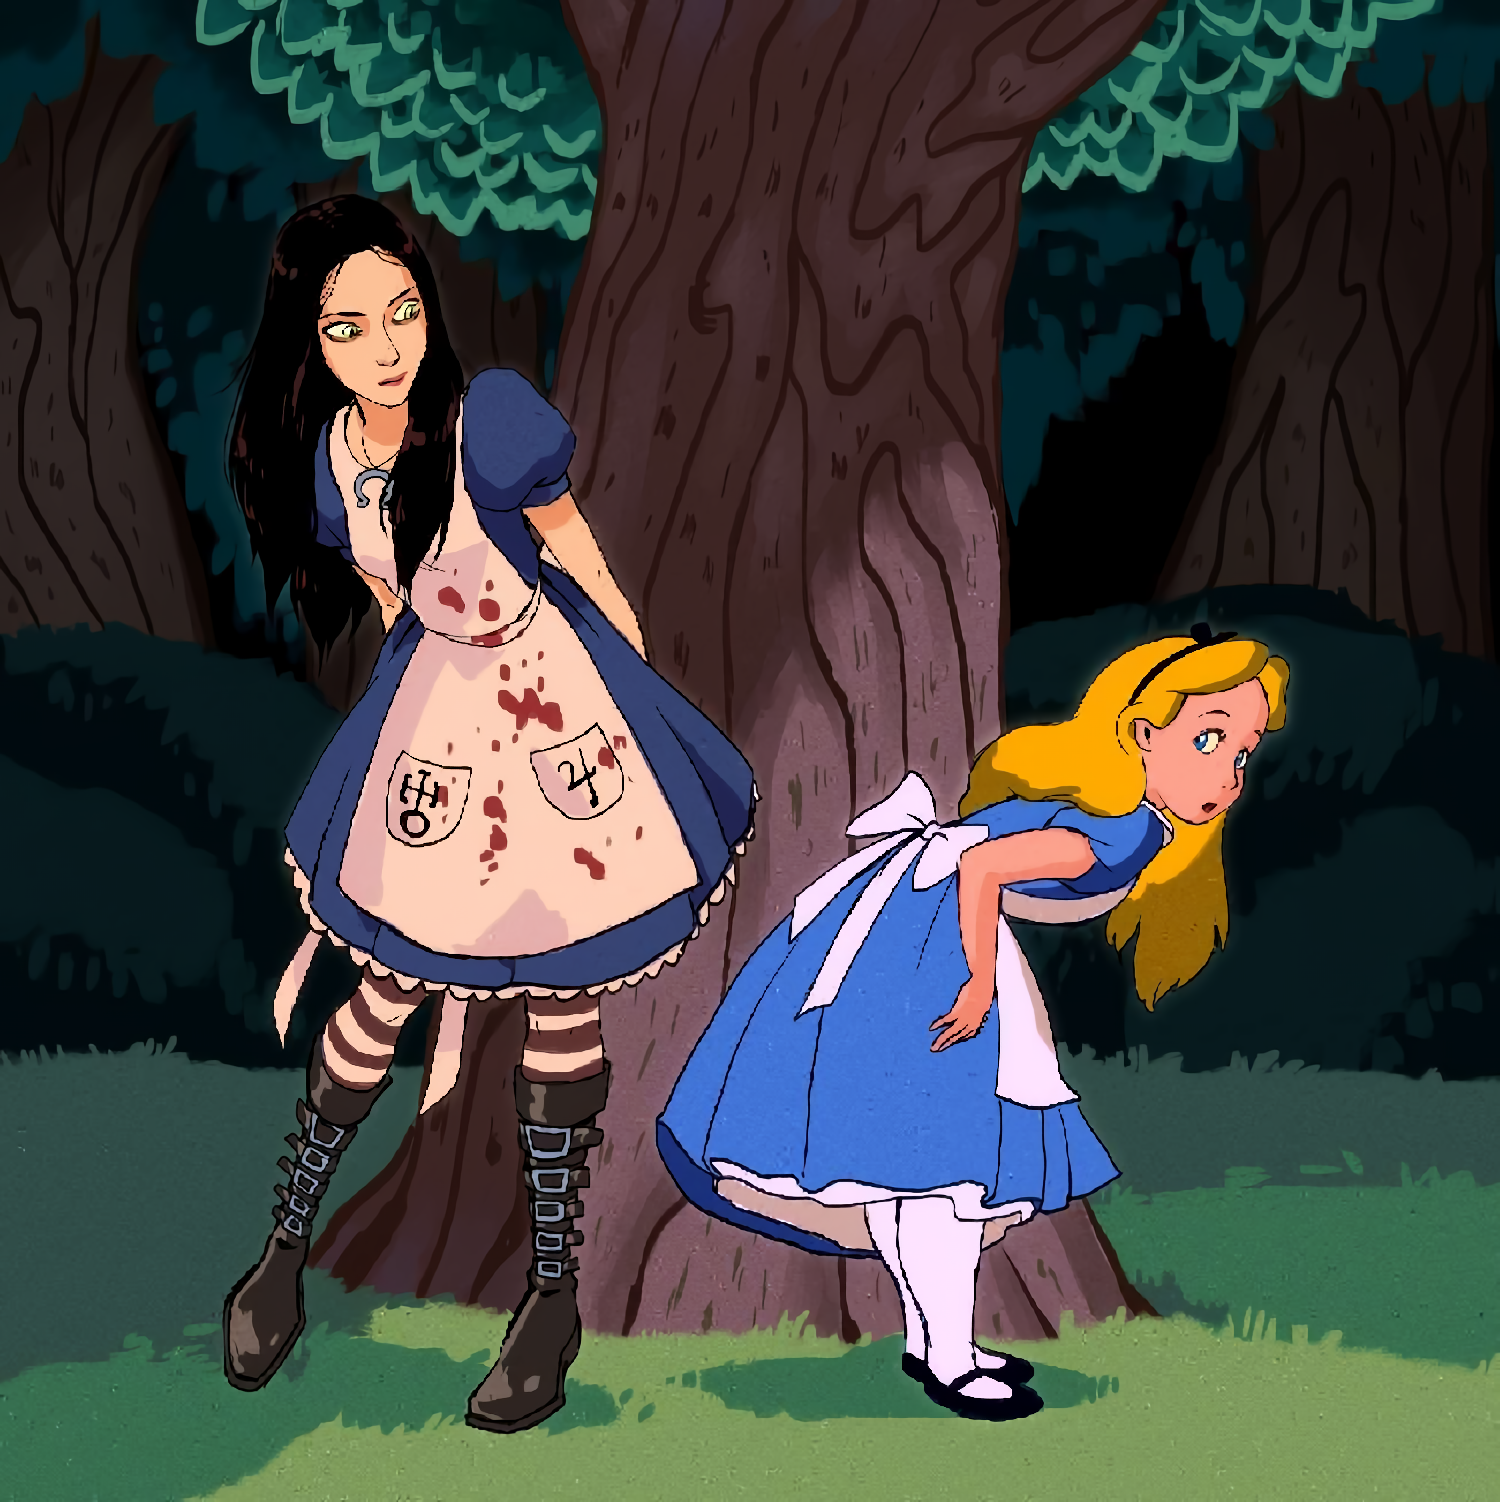
\includegraphics[scale= 0.1]{1/P1/Alice.png}
    \caption{}
    \label{CON1}
\end{figure}

\subsection{Link}
\begin{itemize}
    \item \href{https://github.com/KleperForest/Proyecto_1_Digital_2.git}{GitHub}
    \item \href{https://www.youtube.com/watch?v=z7jWWwueQ_Q}{YouTube}
\end{itemize}